%%
%% The first command in your LaTeX source must be the \documentclass command.
\documentclass[acmsmall,screen,10pt,nonacm]{acmart}
% \renewcommand\footnotetextcopyrightpermission[1]{}
% \settopmatter{printacmref=false}

%% \BibTeX command to typeset BibTeX logo in the docs
\AtBeginDocument{%
  \providecommand\BibTeX{{%
    \normalfont B\kern-0.5em{\scshape i\kern-0.25em b}\kern-0.8em\TeX}}}

% \usepackage[shortcuts]{extdash}
% \usepackage{multirow}
% \usepackage{graphicx}
\usepackage{xcolor}
\usepackage{soul}
\usepackage{listings}
\usepackage{courier}

\let\defaulttexttt\texttt
\renewcommand{\texttt}[1]{\defaulttexttt{\small{#1}}}

\lstset{basicstyle=\footnotesize\ttfamily,breaklines=true,captionpos=b}
\lstset{framextopmargin=50pt,frame=bottomline}

%% Rights management information.  This information is sent to you
%% when you complete the rights form.  These commands have SAMPLE
%% values in them; it is your responsibility as an author to replace
%% the commands and values with those provided to you when you
%% complete the rights form.
% \setcopyright{acmcopyright}
% \copyrightyear{2018}
% \acmYear{2018}
% \acmDOI{10.1145/1122445.1122456}

%% These commands are for a PROCEEDINGS abstract or paper.
\acmConference[Woodstock '18]{Woodstock '18: ACM Symposium on Neural
  Gaze Detection}{June 03--05, 2018}{Woodstock, NY}
\acmBooktitle{Woodstock '18: ACM Symposium on Neural Gaze Detection,
  June 03--05, 2018, Woodstock, NY}
\acmPrice{15.00}
\acmISBN{978-1-4503-XXXX-X/18/06}


%%
%% Submission ID.
%% Use this when submitting an article to a sponsored event. You'll
%% receive a unique submission ID from the organizers
%% of the event, and this ID should be used as the parameter to this command.
%%\acmSubmissionID{123-A56-BU3}

%%
%% The majority of ACM publications use numbered citations and
%% references.  The command \citestyle{authoryear} switches to the
%% "author year" style.
%%
%% If you are preparing content for an event
%% sponsored by ACM SIGGRAPH, you must use the "author year" style of
%% citations and references.
%% Uncommenting
%% the next command will enable that style.
%%\citestyle{acmauthoryear}

%%
%% end of the preamble, start of the body of the document source.
\begin{document}

\definecolor{UoC}{RGB}{137 33 27}
\begin{center}

\includegraphics[scale=0.2]{figures/UoC_logo.png}\\
\textcolor{UoC}{\textbf{UNIVERSITY OF CRETE}}
\vspace{3em}
\end{center}

%%
%% The "title" command has an optional parameter,
%% allowing the author to define a "short title" to be used in page headers.
\title{Impact of Exported Fast Block Storage Devices on the Performance of Managed Big Data Frameworks.}
\subtitle{Thesis submitted in partial fulfilment of the requirements for the degree of Computer Science}

\thanks{\small{This thesis was supervised by Prof. Angelos Bilas, co-supervised by Jane Doe, PhD, Institute of Computer Science, FORTH, and submitted in July 2021}}

%%
%% The "author" command and its associated commands are used to define
%% the authors and their affiliations.
%% Of note is the shared affiliation of the first two authors, and the
%% "authornote" and "authornotemark" commands
%% used to denote shared contribution to the research.
\author{Theodoros Pontzouktzidis}
\affiliation{%
  \department{Computer Science Department}
  \institution{University of Crete}
  \city{Heraklion}
  \country{Greece}
}
\email{csd4336@csd.uoc.gr}

%%
%% By default, the full list of authors will be used in the page
%% headers. Often, this list is too long, and will overlap
%% other information printed in the page headers. This command allows
%% the author to define a more concise list
%% of authors' names for this purpose.
\renewcommand{\shortauthors}{T. Pontzouktzidis}

%%
%% The abstract is a short summary of the work to be presented in the
%% article.
\begin{abstract}
Lorem ipsum dolor sit amet, consectetur adipiscing elit. Nam congue lacus eget quam bibendum pulvinar. Pellentesque sit amet convallis tortor. Vivamus nisi justo, volutpat et quam quis, semper fermentum lectus. Fusce et laoreet erat, at ultricies nibh. Donec malesuada sapien vitae ligula scelerisque tempor. Morbi maximus erat non nulla blandit pulvinar. Vivamus fringilla ipsum pulvinar mi molestie, vel fermentum elit bibendum. Proin turpis est, faucibus vehicula erat a, semper tempus nisi. Praesent ullamcorper mollis porttitor. Suspendisse varius quam arcu, id aliquet turpis rhoncus in. Suspendisse ac lobortis nibh. Curabitur libero ligula, dapibus ut tristique at, porta eu ante. Fusce scelerisque augue lorem, et suscipit felis facilisis nec. Maecenas ullamcorper quam eros, sed euismod neque ullamcorper quis. Quisque consequat eleifend risus posuere laoreet. Nullam tempus velit eu mauris rhoncus, a porta purus mattis.

\end{abstract}

%%
%% The code below is generated by the tool at http://dl.acm.org/ccs.cfm.
%% Please copy and paste the code instead of the example below.
%%
% \begin{CCSXML}
% <ccs2012>
%  <concept>
%   <concept_id>10010520.10010553.10010562</concept_id>
%   <concept_desc>Computer systems organization~Embedded systems</concept_desc>
%   <concept_significance>500</concept_significance>
%  </concept>
%  <concept>
%   <concept_id>10010520.10010575.10010755</concept_id>
%   <concept_desc>Computer systems organization~Redundancy</concept_desc>
%   <concept_significance>300</concept_significance>
%  </concept>
%  <concept>
%   <concept_id>10010520.10010553.10010554</concept_id>
%   <concept_desc>Computer systems organization~Robotics</concept_desc>
%   <concept_significance>100</concept_significance>
%  </concept>
%  <concept>
%   <concept_id>10003033.10003083.10003095</concept_id>
%   <concept_desc>Networks~Network reliability</concept_desc>
%   <concept_significance>100</concept_significance>
%  </concept>
% </ccs2012>
% \end{CCSXML}

% \ccsdesc[500]{Computer systems organization~Embedded systems}
% \ccsdesc[300]{Computer systems organization~Redundancy}
% \ccsdesc{Computer systems organization~Robotics}
% \ccsdesc[100]{Networks~Network reliability}

%%
%% Keywords. The author(s) should pick words that accurately describe
%% the work being presented. Separate the keywords with commas.
% \keywords{datasets, neural networks, gaze detection, text tagging}

%%
%% This command processes the author and affiliation and title
%% information and builds the first part of the formatted document.
\maketitle

\section{Introduction}

Vivamus nec sapien a lorem finibus convallis ut vitae eros. Integer id augue nec ex malesuada scelerisque. In ante velit, imperdiet sed ex non, ultrices laoreet urna. Morbi ut purus neque. Donec vulputate in urna non viverra. Mauris a mi vel augue auctor semper. Nam mollis commodo enim at imperdiet. In hac habitasse platea dictumst. Orci varius natoque penatibus et magnis dis parturient montes, nascetur ridiculus mus. Integer scelerisque, sapien non tristique pharetra, purus purus tempor sem, quis ornare justo magna vitae nisl. Suspendisse potenti. Nulla et bibendum urna. Nam malesuada ac diam ut cursus \cite{lipsum}.

\section{Background}

In this section, we discuss the design of state-of-the art systems that provide
access to remote memory and storage. Specifically, in our study we use Network
Block Device (NBD), NVMe over Fabrics (NVMe-oF), and the Storage Performance
Development Kit (SPDK).

\vspace{1em}
\subsection{TeraHeap}
TeraHeap is a system that eliminates S/D overhead and expensive GC scans for a
large portion of the objects in big data frameworks. TeraHeap enhances the
managed runtime environment, particularly the Java Virtual Machine (JVM). It
introduces a supplementary heap, designed for high-capacity storage, alongside
the primary heap. This secondary heap utilizes fast storage and allows direct
access to objects without the need for serialization or deserialization.
Additionally, TeraHeap minimizes the garbage collection overhead by preventing
the garbage collector from scanning the secondary heap. It takes advantage of
frameworks' capability to designate certain objects for off-heap allocation and
provides them with a hint-based method for relocating these objects to the
secondary heap. 

\subsection{Network Block Device (NBD)}
 Network Block Device (NBD) is a network protocol that can be used to export a block device from a server where the block device resides to a client. There are multiple NBD implementations
 some of them are :
 \begin{itemize}
 \item  \textbf{nbdkit} is a multi-threaded NBD server with a plugin architecture.
 \item  \textbf{libnbd} is a library to aid in writing NBD clients
 \item  \textbf{qemu} contains an \textbf{embedded NBD server}, \textbf{an embedded NBD client}, and \textbf{a standalone NBD server} (qemu-nbd). They maintain a status document of their NBD implementation.
 \item  A \textbf{GEOM gate-based client implementation for FreeBSD} exists. It has not seen any updates since 2018, and only implements the client side (any server should run on FreeBSD unmodified, however).
 \item  A \textbf{Windows} client implementation exists as part of the RBD implementation of Ceph for Windows.
 \item  \textbf{lwNBD} is a NBD server library, targetting bare metal or OS embedded system. It has a plugin architecture.
 \end{itemize}
 We will focus on the Network Block Device (TCP version). We use the TCP version to investigate the overheads added by the TCP protocol stack and compare it with other mechanisms for exporting block devices over the network.
  \begin{figure}[h]
    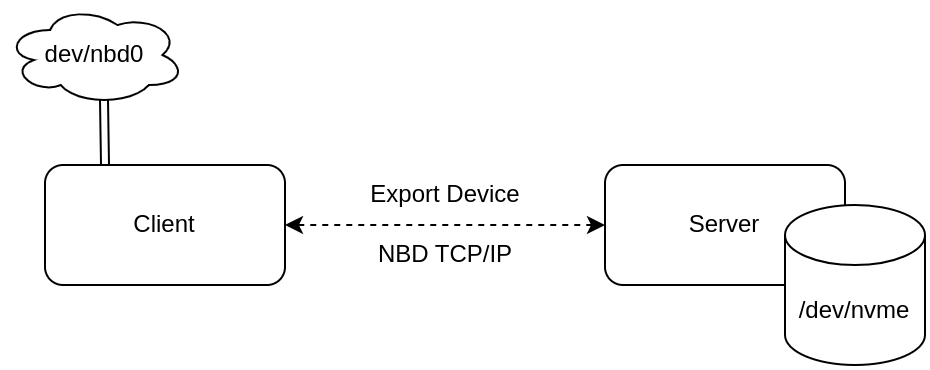
\includegraphics[scale=0.3]{figures/nbd-path.png}\\
    \caption{Overview of an NBD system.}
  \end{figure}
  
With this implementation compiled in the kernel we can use 2 drivers-modules the nbd-client and the nbd-server Figure 1. shows an overview of a NBD system. The nbd-client usually resides in the OS kernel and exposes a block device interface to the rest of the kernel, so that it may appear as an ordinary, directly-attached storage device. The client passes the block requests to the NBD driver where they are encapsulated as NBD network messages and sent to the server via TCP. Finally the User-Space server upon receiving the NBD request issues standard I/O to the relevant block device and then responds Figure 2. shows a more in depth I/O path using NBD TCP Version. 

  \begin{figure}[h]
    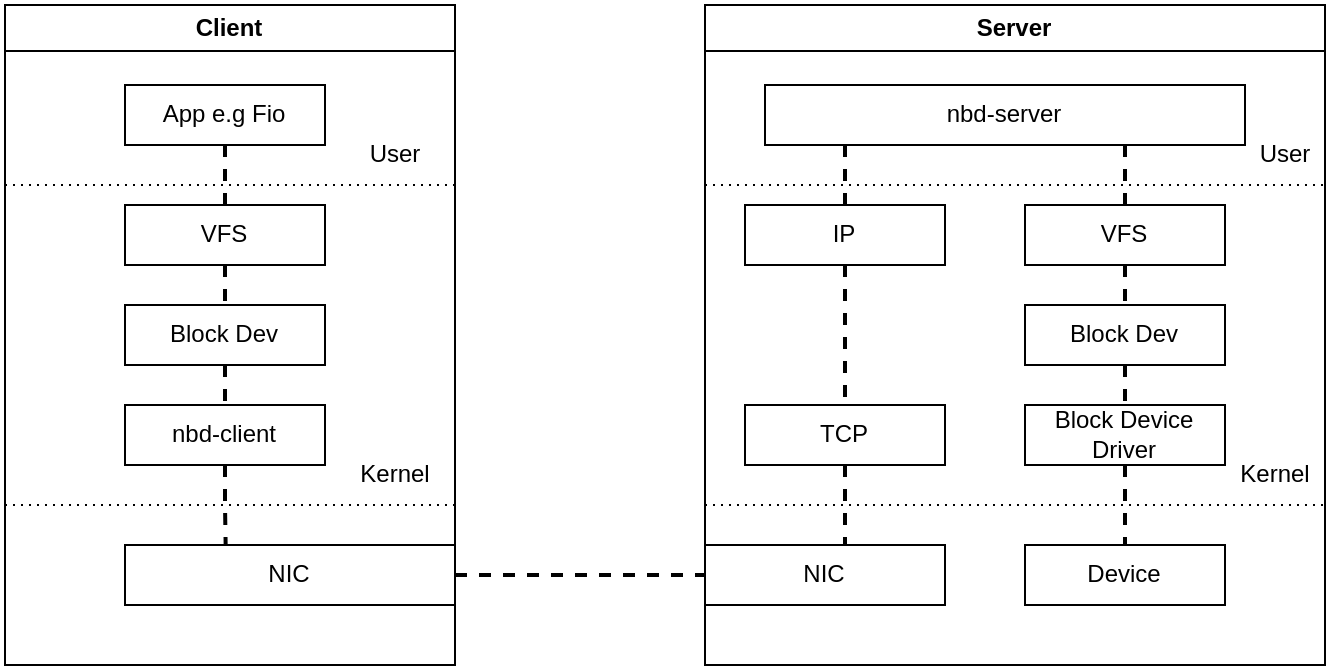
\includegraphics[scale=0.25]{figures/nbd-path2.png}\\
    \caption{I/O Path of NBD system.}
  \end{figure}

\vspace{1em}
\subsection{NVMe over Fabrics (NVMe-oF)}
NVMe over Fabrics (NVMe-oF) is a protocol specification designed for connecting
hosts to storage systems over a network using the NVMe protocol. It enables the
transfer of data between a host computer and a target solid-state storage device
or system through network communication. This protocol utilizes NVMe
message-based commands to facilitate data transfers, supporting various
networking technologies such as Ethernet, Fibre Channel (FC), and InfiniBand.

\vspace{1em}
\subsection{Storage Performance Development Kit (SPDK)}
The Storage Performance Development Kit (SPDK) is a versatile toolkit tailored
for crafting high-performance, scalable storage applications in user-mode
environments. Its architecture revolves around several core principles aimed at
optimizing performance like User-Space Drivers, Polling Mechanism and lockless
I/O handling. At its foundation, SPDK features a user-space, asynchronous NVMe
driver designed for zero-copy, highly parallel access to SSDs. This driver,
presented as a C library with a simple public header, facilitates seamless
integration for developers. Additionally, SPDK offers a user-space block stack
library mirroring OS functionalities, including storage device interface
unification, queue management for resource constraints, and logical volume
administration. SPDK extends its capabilities with NVMe-oF, iSCSI, and vhost
servers built atop these foundational components. 

SPDK operates entirely in user space, bypassing the kernel entirely for I/O operations. By eliminating the overhead of kernel context switches and system calls, SPDK can achieve significantly higher performance and lower latency compared to traditional storage solutions that rely on kernel-level operations. Memory management in SPDK is highly optimized, utilizing techniques such as large memory buffers, memory pooling, and zero-copy operations. Large memory buffers are allocated upfront, often using huge pages, to ensure contiguous memory allocation and reduce fragmentation. Memory pooling minimizes the overhead of dynamic memory allocation and deallocation, while zero-copy operations eliminate unnecessary data copies, further enhancing performance. Integration with the Data Plane Development Kit (DPDK) enhances SPDK's performance by leveraging DPDK's efficient packet processing capabilities for networked storage solutions. This integration enables SPDK to handle network I/O with minimal overhead, ensuring high throughput and low latency for storage applications deployed in networked environments. SPDK's support for NVMe-oF extends the NVMe protocol over fabrics, allowing remote access to NVMe storage devices with minimal overhead. This involves sophisticated handling of NVMe commands and data over high-speed networks, optimizing performance and scalability for distributed storage solutions. 

Figure 3. Shows the overview of the SPDK NVMe-oF Target-Initiator system. The process begins with the target unbinding traditional kernel drivers associated with the block device and binding them with SPDK's user-space drivers. This step grants SPDK exclusive control over the block device, enabling optimized I/O handling and performance. Subsequently, the block device, now under the control of SPDK in user space, is exported to the network using the NVMe-oF protocol specification, facilitated by RDMA. RDMA plays a pivotal role in enabling high-speed, low-latency data transfers over the network, allowing direct access to remote system memory without CPU involvement. This exportation process ensures efficient data transmission between the NVMe target and initiator. Additionally, SPDK supports kernel initiators, allowing traditional kernel-based applications to connect to SPDK NVMe-oF targets. Through this mechanism, kernel initiators can access the SPDK-exported block device over the network using standard device nodes such as /dev/nvme.
\begin{figure}[h]
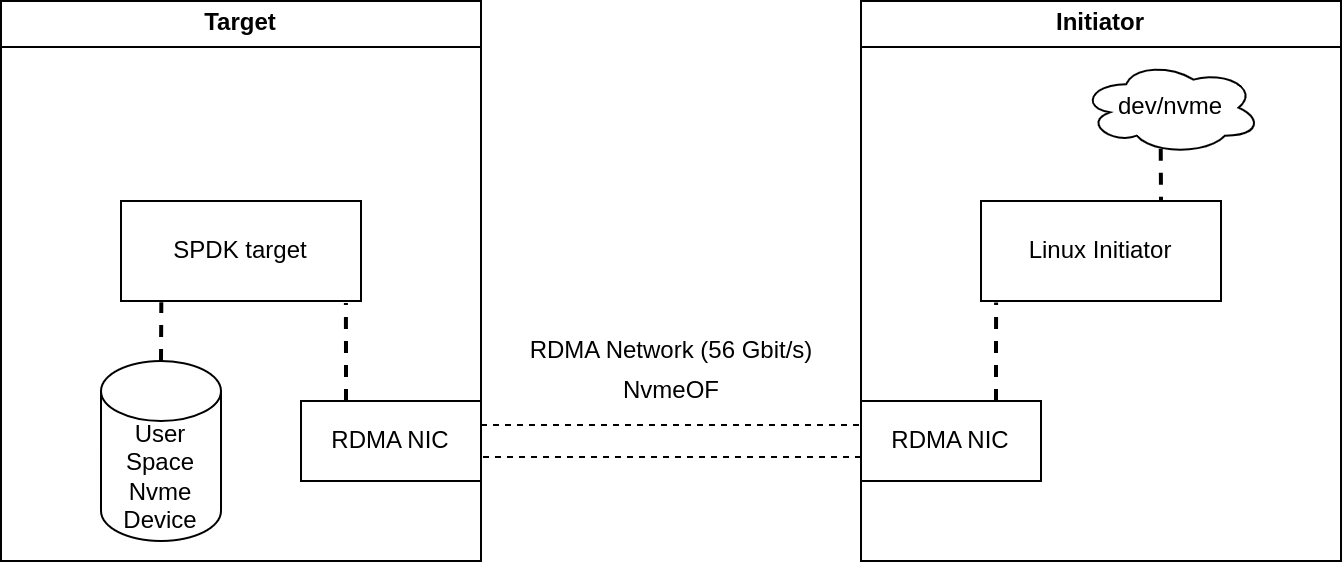
\includegraphics[scale=0.25]{figures/spdk-target.png}\\
\caption{Overview of SPDK NvmeOF Target-Initiator system.}
\end{figure}

\vspace{8em}
\subsection{FIO}
\note{jk: move this to the methodology where we are going to discuss about how
we run the experiments}
Flexible I/O (FIO) Tester, is a widely used open-source tool in the
Linux ecosystem for benchmarking and testing various I/O (input/output)
workloads on storage devices. FIO offers extensive customization options,
enabling users to specify parameters such as block size, I/O pattern
(sequential, random), read/write ratio, queue depth, and concurrency. This
flexibility makes it suitable for evaluating different storage scenarios,
including HDDs, SSDs, NVMe drives, and network storage systems. Additionally,
FIO provides detailed output reports, allowing users to analyze metrics such as
throughput, IOPS (input/output operations per second), latency, and CPU
utilization. We will use FIO for generating I/O 
\vspace{1em}

\section{Design and implementation}

Nunc neque quam, scelerisque vel justo non, viverra ornare dolor. Maecenas nisl ligula, efficitur eu justo at, gravida semper velit. Maecenas quis convallis velit, et elementum justo. Duis aliquet, risus eu posuere ornare, sem metus consequat neque, vehicula dignissim justo dolor id justo. Aenean accumsan pulvinar justo id fringilla. In ultrices felis tempus varius consequat. Mauris scelerisque massa pharetra tristique scelerisque. Vestibulum elit tellus, pellentesque eget orci sit amet, venenatis hendrerit arcu. Pellentesque eu justo mauris. Cras vel dapibus ipsum. Praesent nec malesuada urna, sit amet lacinia velit. Vivamus pharetra volutpat hendrerit. Curabitur tristique ut justo id dignissim. Donec tempor gravida ultricies.

Sed ac pharetra quam. Praesent sed fermentum ante, et congue arcu. Suspendisse potenti. Vestibulum dolor enim, faucibus vitae blandit in, hendrerit eu dui. Sed fringilla sed sem vel dapibus. Cras pellentesque neque ligula, ac fermentum enim posuere at. In hac habitasse platea dictumst. Cras vitae tellus at orci imperdiet euismod. Ut ultrices sollicitudin efficitur. Quisque porttitor eget nisi non dapibus. Aenean molestie velit quis efficitur venenatis. Morbi ac purus ac tortor maximus fringilla quis ut arcu. Nulla sollicitudin id velit congue laoreet.

\section{Conclusion}

Praesent in aliquet metus. Nullam et tellus elit. In ornare dui et lectus luctus, vel interdum nisi rhoncus. Sed ultricies libero sed velit pretium, vel interdum dui varius. Nullam quis luctus risus. Donec nulla quam, suscipit eu scelerisque in, gravida at dolor. Duis feugiat, elit in consectetur egestas, neque libero vestibulum libero, vel congue dui dui a nunc. Morbi ut mattis neque. Nullam tempus nunc eget urna condimentum semper.

\begin{acks}
The author would like to thank Numerius Negidius for his valuable comments and suggestions during this work.
\end{acks}


\bibliographystyle{ACM-Reference-Format}
\bibliography{references}

\end{document}
